\chapter{无人机辅助 MEC 系统中的轨迹与任务卸载协同优化算法}

\label{cha:system-model}

\section{系统模型与问题建模}

\label{sec:system-problem-modeling}

本节建立无人机辅助移动边缘计算（UAV-assisted mobile edge computing, UAV-MEC）系统的数学模型，并在此基础上形式化本文需要求解的轨迹与任务卸载协同优化问题。建模过程遵循系统运行的自然顺序：首先描述 UAV、UE 与 MBS 构成的网络场景，其次刻画无线链路速率和请求生成过程，然后根据不同卸载位置计算服务时延和能耗，最后将长期奖励最大化问题写成带物理约束和服务质量约束的优化问题。

\subsection{网络与时隙模型}
\label{sec:network-model}

本文考虑一个由 $N=5$ 架 UAV、$M=100$ 个 UE 和一个宏基站（macro base station, MBS）构成的 UAV-MEC 系统。UAV 在固定高度 $H=100$ m 飞行，并在 $700 \times 700$ m$^2$ 的水平区域内为地面用户提供覆盖、计算卸载和无线能量传输服务。MBS 作为远端稳定计算节点，在 UAV 本地计算资源或 UAV 间协作资源不足时提供回退执行能力，但过度依赖 MBS 会增加回传压力并造成系统负载集中。因此，本文需要同时决定 UAV 的空间位置和服务请求的执行位置。

系统时间被划分为长度为 $\tau=1$s 的离散时隙，一个 episode 包含 $T=1000$ 个时隙。记第 $n$ 个时隙 UAV $i$ 的水平位置为 $\mathbf{q}_n^{(i)}=(x_n^{(i)},y_n^{(i)})$，其中 $i\in\{0,1,\ldots,N-1\}$。UAV 的覆盖半径为 $R_c=100$ m，最大飞行速度为 $v_{max}=15$ m/s，任意两架 UAV 之间需保持不低于 $d_{min}=200$ m 的安全间距。系统主要包含 UE-UAV 上行链路、UAV-UAV 协作链路和 UAV-MBS 回传链路，如图 \ref{fig:system-model} 所示。后续轨迹控制会改变 UE 与 UAV 的相对距离，从而影响链路速率、任务时延、能耗以及用户覆盖公平性。

\begin{figure}[!htbp]
    \centering
    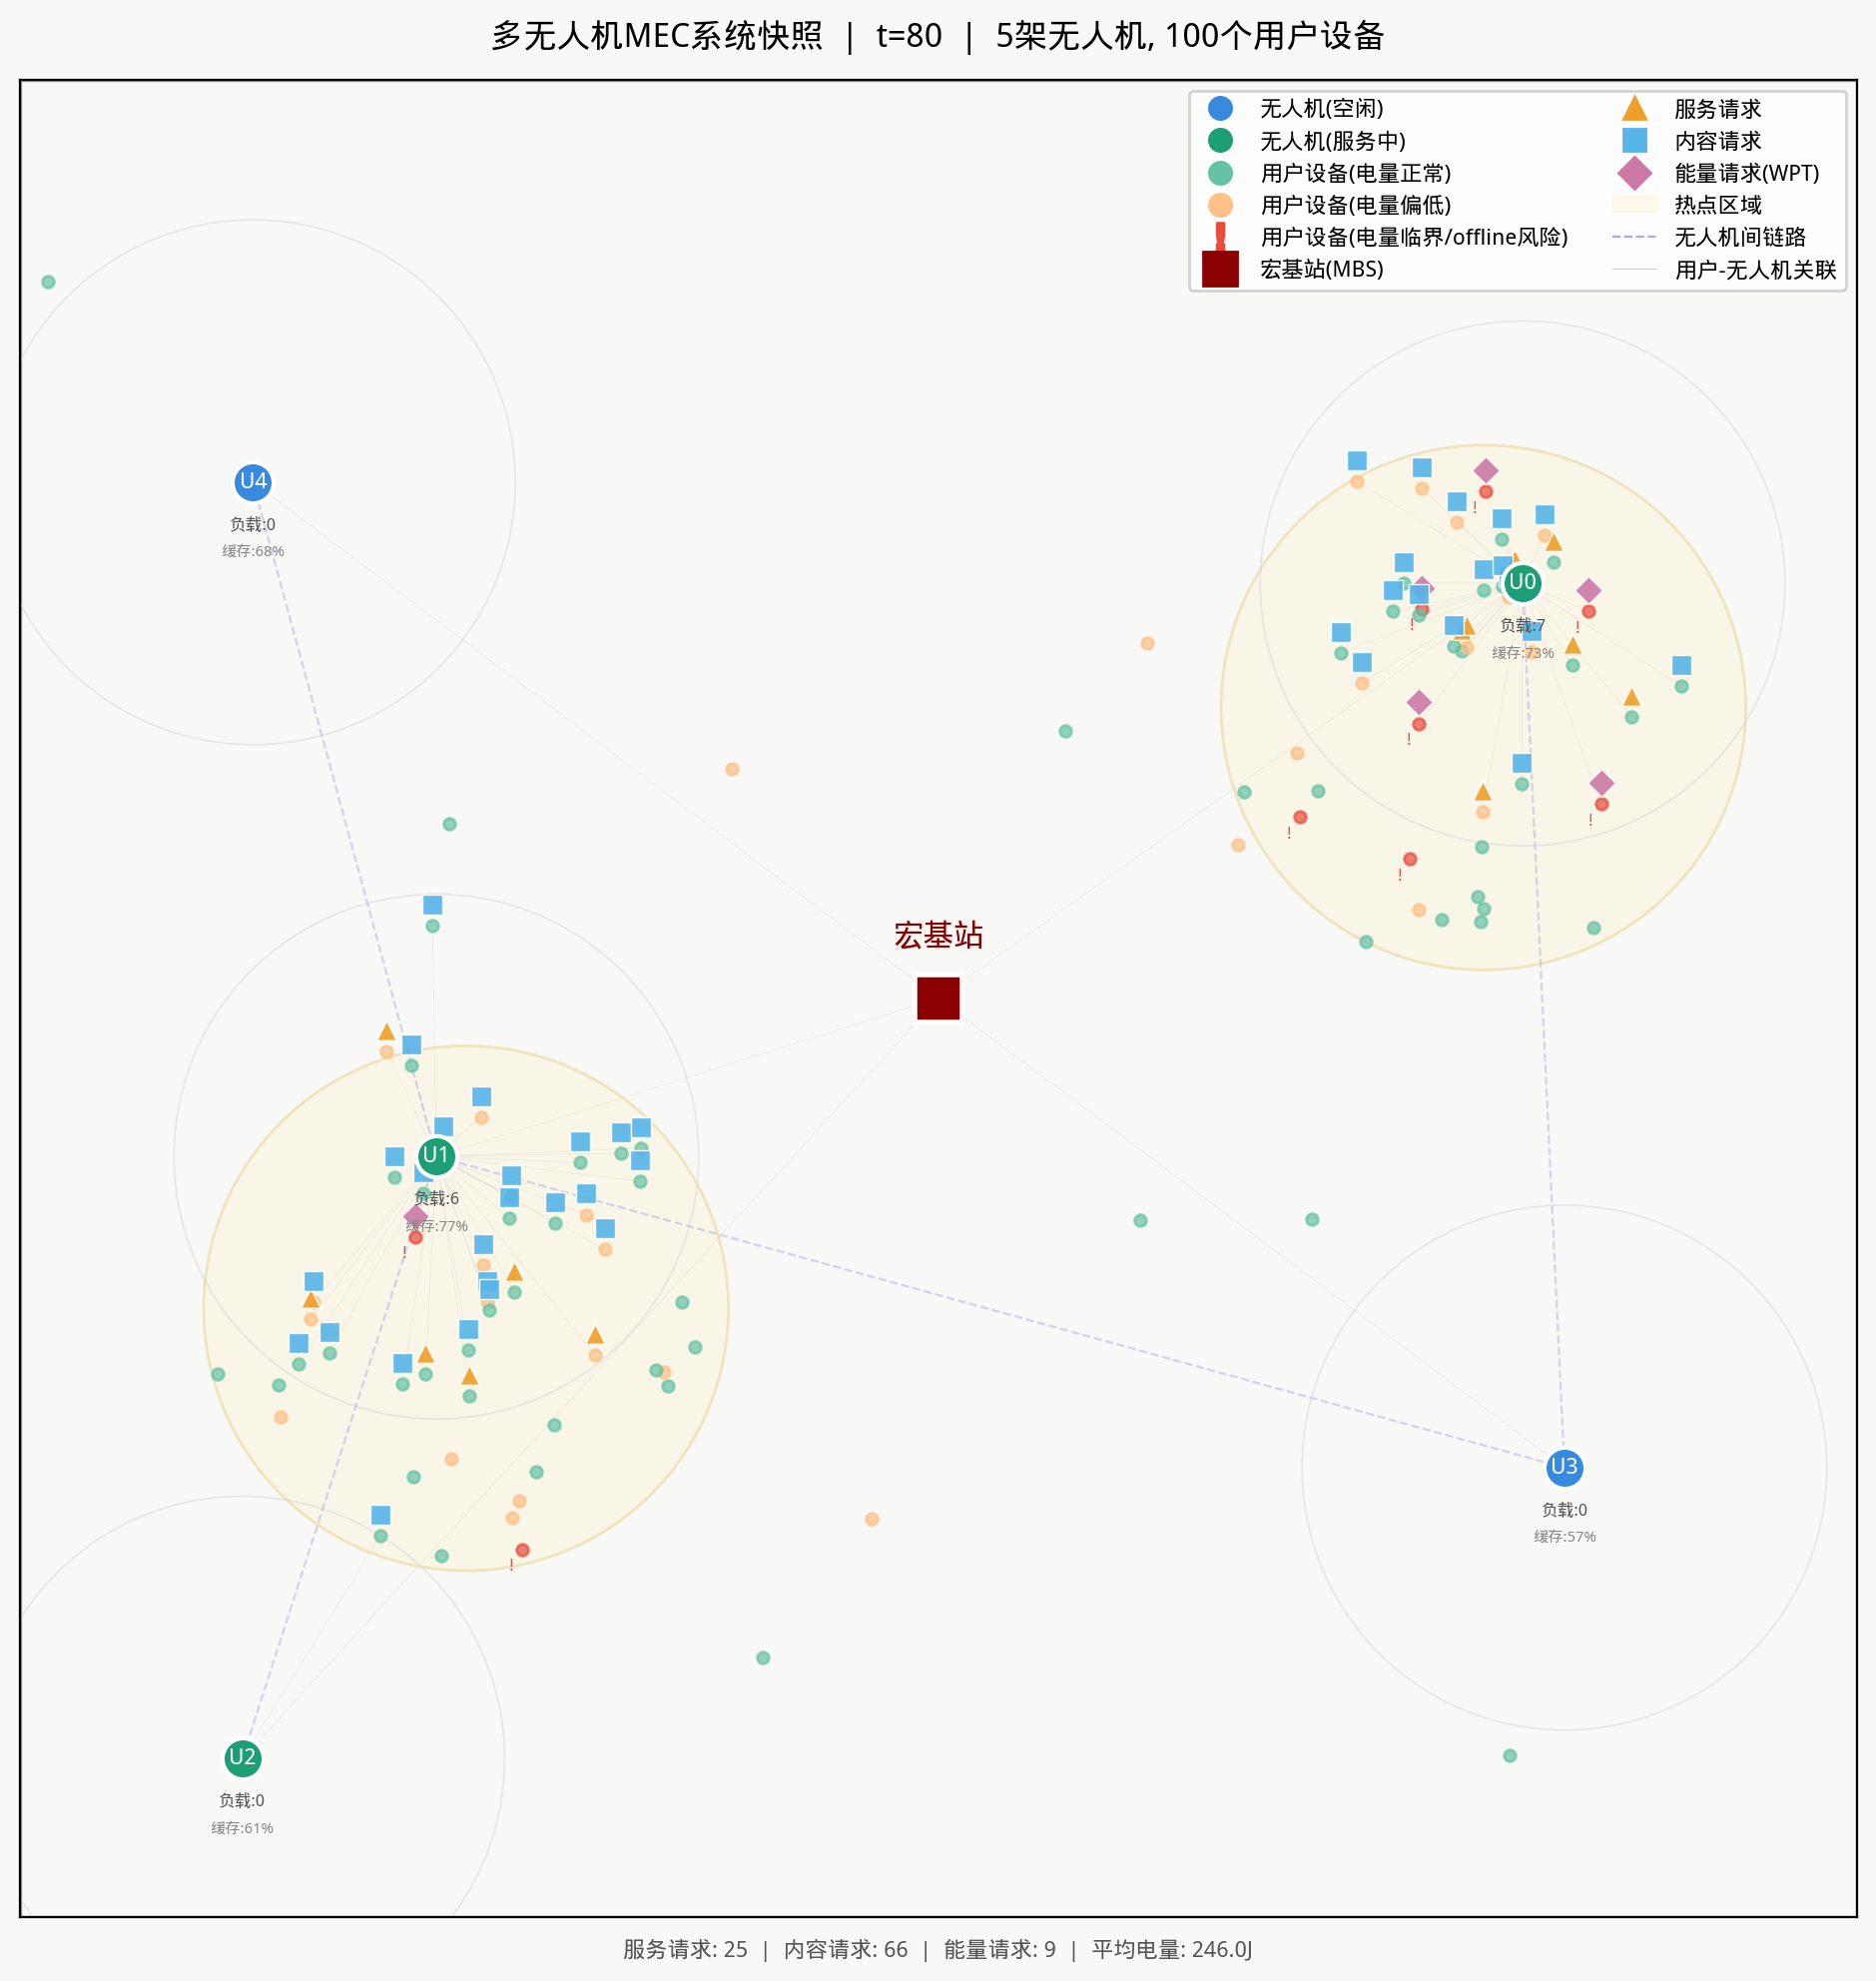
\includegraphics[width=0.85\textwidth]{docs/figures/fig_system_snapshot.png}
    \bicaption{系统场景与链路模型}{System scenario and link model}
    \label{fig:system-model}
\end{figure}

\subsection{通信链路模型}
\label{sec:communication-model}

在上述网络中，无线链路质量首先由通信距离决定。本文采用自由空间路径损耗模型描述视距（Line-of-Sight, LoS）信道，距离为 $d$ 时的信道增益定义为
\begin{equation}
    g(d) = \frac{\beta_0}{d^2},
    \label{eq:channel-gain}
\end{equation}
其中 $\beta_0$ 为参考距离 1 m 处的信道功率增益。根据香农公式，给定带宽 $B$、发射功率 $P_{tx}$ 和噪声功率 $\sigma^2$ 时，链路传输速率可写为
\begin{equation}
    R = B \cdot \log_2\left(1 + \frac{P_{tx} \cdot g(d)}{\sigma^2}\right).
    \label{eq:shannon}
\end{equation}
该表达式统一用于刻画 UE-UAV、UAV-UAV 和 UAV-MBS 链路，其中 UAV-MBS 回传链路使用独立带宽 $B_{backhaul}$。由于仿真实现中请求大小和文件大小以 bytes 记录，而链路速率以 bit/s 表示，传输大小为 $D$ bytes 的数据所需时间统一为
\begin{equation}
    T_{tx} = \frac{8 \cdot D}{R}.
    \label{eq:tx-delay}
\end{equation}
式中 $8\times$ 因子完成 bytes 到 bits 的单位转换。由此可见，UAV 轨迹不仅决定覆盖关系，也直接通过距离影响传输速率和后续服务时延。

\subsection{请求生成与卸载决策}
\label{sec:task-model}
\label{subsec:request-types}
\label{subsec:request-arrival}
\label{subsec:offloading-decision}

系统中共有 $S=25$ 类服务和 $K=50$ 类内容文件，分别记为服务集合 $\mathcal{S}=\{0,1,\ldots,S-1\}$ 和内容集合 $\mathcal{K}=\{S,S+1,\ldots,S+K-1\}$。总文件集合为 $\mathcal{F}=\mathcal{S}\cup\mathcal{K}$，且 $|\mathcal{F}|=75$。每个文件 $f\in\mathcal{F}$ 具有固定存储大小 $L_f$（bytes），其中 $L_f\in[10^6,5\times10^6]$ bytes；每个服务类型 $s\in\mathcal{S}$ 具有计算强度 $\omega_s$（cycles/byte），取值范围为 $\omega_s\in[1200,2800]$。

每个 UE 在每个时隙至多生成一个请求。若 UE 当前电池水平 $B_{ue}$ 低于临界阈值 $B_{low}$，该 UE 优先生成能量请求，并暂停本轮服务请求以降低自身能耗；否则，UE 从 $\mathcal{F}$ 中按照 Zipf 分布选择一个文件或服务。设文件 $f$ 的流行度排名为 $\text{rank}(f)$，则其被选择的概率为
\begin{equation}
    P(f) = \frac{1/\text{rank}(f)^\alpha}{\sum_{f'=0}^{|\mathcal{F}|-1} 1/\text{rank}(f')^\alpha},
    \label{eq:zipf}
\end{equation}
其中 $\alpha$ 控制请求流行度的集中程度。若被选中的 ID 属于服务集合 $\mathcal{S}$，则生成计算密集型服务请求；若属于内容集合 $\mathcal{K}$，则生成内容请求。

一个服务请求形式化表示为
\begin{equation}
    \mathcal{T}_m = \left(D_m, \omega_{s_m}, T_m^{dl}, p_m\right),
    \label{eq:service-request}
\end{equation}
其中 $D_m\in[D_{min},D_{max}]$ 为输入数据量，$\omega_{s_m}$ 为服务类型 $s_m$ 的计算强度，$T_m^{dl}\in[T_{dl}^{min},T_{dl}^{max}]$ 为截止时间，$p_m\in\{1,2,3\}$ 为优先级。该服务请求所需 CPU 周期数为
\begin{equation}
    C_m = \omega_{s_m} \cdot D_m \quad (\text{cycles}).
    \label{eq:computation-workload}
\end{equation}
内容请求不涉及计算卸载，仅需完成内容文件传输，可表示为
\begin{equation}
    \mathcal{C}_m = (f_m, L_{f_m}),
    \label{eq:content-request}
\end{equation}
其中 $f_m\in\mathcal{K}$ 为请求的内容文件 ID，$L_{f_m}$ 为文件大小。

设 UAV $i$ 在当前时隙关联的服务请求集合为 $\mathcal{M}_i$，且 $|\mathcal{M}_i|\leq M_i^{max}$。对于任意 $m\in\mathcal{M}_i$，系统需要为其选择执行位置，即离散卸载决策
\begin{equation}
    a_m \in \mathcal{A} = \{0, 1, 2, \ldots, N\}.
    \label{eq:offload-action}
\end{equation}
其中 $a_m=0$ 表示在当前 UAV 本地执行，$a_m=1$ 表示通过回传链路卸载至 MBS 执行，$a_m=2+i$ 表示卸载至协作 UAV $i$ 执行。该动作空间与第 \ref{sec:lower-layer} 节的下层 MARL 策略一致，当前 $N=5$ 时共有 $N+2=7$ 个卸载动作。至此，轨迹变量决定 UE 与 UAV 的连接质量，而卸载变量决定任务的执行路径，二者共同影响服务时延和系统能耗。

\subsection{时延与能耗模型}
\label{sec:computation-model}
\label{subsec:latency-model}
\label{subsec:uav-energy}
\label{subsec:comm-energy}

对于服务请求 $\mathcal{T}_m$，总处理时延由上行传输、可能的协作/回传传输、服务或文件获取以及计算执行共同构成。本文假设计算结果数据量远小于输入数据量，因此结果回传时延可忽略。若请求在当前 UAV 本地执行，则时延为
\begin{equation}
    T_{local} = T_{tx}^{ue-uav} + T_{fetch}^{local} + T_{comp}^{uav}
    = \frac{8D_m}{R_{ue-uav}} + T_{fetch}^{local} + \frac{C_m}{f_{uav}},
    \label{eq:local-latency}
\end{equation}
其中 $R_{ue-uav}$ 为 UE-UAV 上行速率，$f_{uav}$ 为 UAV 计算能力，$T_{fetch}^{local}$ 表示本地 UAV 未缓存对应服务或文件时从 MBS 获取资源产生的额外时延，缓存命中时该项为 0。

若请求卸载至协作 UAV 执行，则除 UE 到当前 UAV 的上行传输外，还需要经过 UAV-UAV 协作链路转发，其时延为
\begin{equation}
    T_{coop} = \frac{8D_m}{R_{ue-uav}} + \frac{8D_m}{R_{uav-uav}} + T_{fetch}^{coop} + \frac{C_m}{f_{coop}},
    \label{eq:coop-latency}
\end{equation}
其中 $R_{uav-uav}$ 为 UAV 间协作链路速率，$f_{coop}$ 为协作 UAV 的计算能力，$T_{fetch}^{coop}$ 为协作 UAV 未缓存所需资源时产生的额外获取时延。若请求卸载至 MBS 执行，则时延为
\begin{equation}
    T_{mbs} = \frac{8D_m}{R_{ue-uav}} + \frac{8D_m}{R_{backhaul}} + \frac{C_m}{f_{mbs}},
    \label{eq:mbs-latency}
\end{equation}
其中 $R_{backhaul}$ 为 UAV-MBS 回传链路速率，$f_{mbs}=200\times10^9$ cycles/s 为 MBS 固定计算能力。上述三类路径对应图 \ref{fig:latency-process} 中的服务处理流程，并构成后续 DSR 和归一化时延指标的计算基础。

\begin{figure}[!htbp]
    \centering
    
\includegraphics[width=0.85\textwidth]{docs/figures/fig_latency_process.png}
    \bicaption{时延处理流程}{Latency processing flow}
    \label{fig:latency-process}
\end{figure}

在能耗方面，UAV 侧能耗主要由计算、通信、飞行和 WPT 发射组成。计算能耗采用 CMOS 动态功耗模型估计：
\begin{equation}
    E_{comp} = K_{cpu} \cdot C_m \cdot f^2,
    \label{eq:comp-energy}
\end{equation}
其中 $K_{cpu}=10^{-27}$ 为 CPU 电容系数，$f$ 为执行该请求的计算节点频率。每架 UAV 的计算能力 $f_{uav}$ 在 $40\times10^9$ 至 $90\times10^9$ cycles/s 之间随机生成。通信能耗由通信功率与传输时长决定：
\begin{equation}
    E_{comm} = P_{comm} \cdot T_{tx}.
    \label{eq:comm-energy}
\end{equation}
其中 UE 发射功率为 $P_{ue}=0.5$ W，UAV 通信发射和接收功率分别为 0.5 W 和 0.1 W，UAV-MBS 回传发射功率为 0.5 W。

\subsection{电池、无线能量传输与飞行能耗模型}
\label{sec:battery-wpt}
\label{subsec:battery-model}
\label{subsec:wpt}
\label{sec:flight-energy}

由于本文关注长期服务连续性，仅考虑任务时延和 UAV 能耗是不够的。UE 电池状态会影响请求类型和离线率，而 UAV 轨迹移动本身也会消耗大量能量。因此，系统还需要描述 UE 电池动态、无线能量传输（wireless power transfer, WPT）和 UAV 飞行能耗。

每个 UE 配备容量为 $B_{max}=500$ J 的电池。每个时隙结束后，UE 电池状态更新为
\begin{equation}
    B_{t+1} = \min\left(B_{max}, \; B_t - E_{static} - E_{tx} \cdot \mathbb{1}[\text{transmit}] - E_{rx} \cdot \mathbb{1}[\text{receive}] + E_{harv}\right),
    \label{eq:battery-dynamics}
\end{equation}
其中 $E_{static}=P_{static}\cdot\tau=0.01$ J 为待机能耗，$E_{tx}=P_{ue}\cdot T_{tx}$ 为发射能耗，$E_{rx}$ 为接收内容或计算结果时产生的接收能耗，$E_{harv}$ 为无线能量采集量。当 $B_{ue}<B_{low}=0.1B_{max}=50$ J 时，UE 进入离线状态，不再生成服务请求，而是产生紧急能量请求。系统离线率定义为
\begin{equation}
    O = \frac{|\{ue \mid B_{ue} < B_{low}\}|}{M}.
    \label{eq:offline-rate}
\end{equation}

UAV 可对覆盖范围内的低电量 UE 进行 WPT。单个 UE 在一个时隙内可采集的能量为
\begin{equation}
    E_{harv} = \eta \cdot P_{wpt} \cdot G \cdot g(d) \cdot \tau,
    \label{eq:wpt-energy}
\end{equation}
其中 $\eta=0.8$ 为能量采集效率，$P_{wpt}=50$ W 为 WPT 发射功率，$G=5\times10^5$ 为等效采集增益，$g(d)$ 为式 (\ref{eq:channel-gain}) 中的信道增益。

UAV 飞行能耗由移动时间和悬停时间共同决定。若 UAV 在当前时隙内移动距离为 $d_{moved}$，则飞行能耗为
\begin{equation}
    E_{fly} = P_{move} \cdot t_{moving} + P_{hover} \cdot t_{hovering},
    \label{eq:flight-energy}
\end{equation}
\begin{equation}
    t_{moving} = \frac{d_{moved}}{v_{max}}, \quad t_{hovering} = \tau - t_{moving}.
    \label{eq:time-decomposition}
\end{equation}
其中 $P_{move}=300$ W，$P_{hover}=150$ W。全速飞行时 $E_{fly}=300$ J，悬停时 $E_{fly}=150$ J。综合上述各项，UAV 侧单步总能耗定义为
\begin{equation}
    E_{total} = \sum_{i=0}^{N-1} \left(E_{fly}^{(i)} + E_{comp}^{(i)} + E_{comm}^{(i)} + E_{wpt}^{(i)}\right),
    \label{eq:total-energy}
\end{equation}
其中 $E_{wpt}^{(i)}=P_{wpt}\cdot\tau\cdot\mathbb{1}[\text{has energy request}]$ 表示 UAV $i$ 在该时隙执行 WPT 时产生的发射能耗。至此，系统性能由时延、能耗、服务公平性和 UE 电池状态共同决定。

\subsection{优化目标与约束条件}
\label{sec:optimization-objective}
\label{sec:constraints}

基于以上模型，本文目标是在动态请求到达、无线链路变化和 UE 电池演化的条件下，联合优化 UAV 轨迹控制策略 $\pi^{upper}$ 与请求卸载策略 $\pi^{lower}$，使系统长期综合奖励最大化：
\begin{equation}
    \max_{\pi^{upper}, \pi^{lower}} \mathbb{E}\left[\sum_{t=0}^{T-1} \gamma^t R_t\right].
    \label{eq:optimization}
\end{equation}
其中 $\gamma$ 为折扣因子，$R_t$ 为第 $t$ 个时隙的系统级综合奖励。考虑到本文同时关注覆盖公平性、时延、能耗、UE 离线率、截止时间满足率和 MBS 负载，奖励函数定义为
\begin{equation}
    R_t = W_J \cdot J_t - W_L \cdot \bar{L}_t - W_E \cdot \bar{E}_t - W_O \cdot O_t + W_{DSR} \cdot DSR_t - W_M \cdot M_t.
    \label{eq:reward}
\end{equation}
式中，$J_t\in[0,1]$ 为 Jain 公平性指数，定义为 $J_t=\frac{(\sum_{i=1}^M x_i)^2}{M\sum_{i=1}^M x_i^2}$，其中 $x_i$ 表示 UE $i$ 的服务覆盖水平；$\bar{L}_t$ 为以 $M\cdot T_{penalty}$ 归一化的系统时延，$T_{penalty}=20$s 为未服务请求惩罚时延；$\bar{E}_t$ 为以 $N\cdot E_{ref}$ 归一化的 UAV 侧能耗；$O_t$ 为式 (\ref{eq:offline-rate}) 给出的 UE 离线率。

截止时间满足率（deadline satisfaction rate, DSR）刻画已分配服务请求中满足截止时间约束的比例，定义为
\begin{equation}
    DSR_t = \frac{|\{m \mid \mathcal{T}_m \in \mathcal{S}, \; a_m \neq \varnothing, \; L_m \leq T_m^{dl}\}|}{|\{m \mid \mathcal{T}_m \in \mathcal{S}\}|},
    \label{eq:dsr-definition}
\end{equation}
其中 $L_m$ 为请求 $m$ 的实际处理时延，$a_m\neq\varnothing$ 表示该请求已被分配执行。MBS 负载比例用于约束系统对远端计算节点的依赖程度，定义为
\begin{equation}
    M_t = \frac{|\{m \mid \mathcal{T}_m \in \mathcal{S}, \; a_m = 1\}|}{|\{m \mid \mathcal{T}_m \in \mathcal{S}, \; a_m \neq \varnothing\}|}.
    \label{eq:mbs-load-definition}
\end{equation}
本文采用的系统级权重为 $W_J=1.0$、$W_L=1.0$、$W_E=0.5$、$W_O=5.0$、$W_{DSR}=1.0$、$W_M=0.5$。当 UAV 发生碰撞或越界时，环境额外施加 $-10$ 惩罚；最终 reward 乘以 0.1 缩放因子，以稳定 MARL 训练过程中的数值范围。

上述优化问题需要满足以下约束。首先，UAV 必须始终位于服务区域内：
\begin{equation}
    \mathbf{q}_n^{(i)} \in [0, W] \times [0, W], \quad \forall i \in \{0, 1, \ldots, N-1\}, \; \forall n,
    \label{eq:constraint-space}
\end{equation}
其中 $W=700$m。其次，任意时隙内 UAV 的位移不得超过最大飞行距离：
\begin{equation}
    \|\mathbf{q}_{n+1}^{(i)} - \mathbf{q}_n^{(i)}\| \leq v_{max} \cdot \tau, \quad \forall i \in \{0, \ldots, N-1\}, \; \forall n.
    \label{eq:constraint-speed}
\end{equation}
任意两架 UAV 之间还需满足安全间距约束：
\begin{equation}
    \|\mathbf{q}_n^{(i)} - \mathbf{q}_n^{(j)}\| \geq d_{min}, \quad \forall i \neq j, \; i, j \in \{0, \ldots, N-1\}, \; \forall n.
    \label{eq:constraint-separation}
\end{equation}
对于每个服务请求，其卸载动作必须属于离散动作空间：
\begin{equation}
    a_m \in \{0, 1, 2, \ldots, N\}, \quad \forall m \in \mathcal{M}_i.
    \label{eq:constraint-offload}
\end{equation}
最后，为避免策略单纯追求能耗或短期奖励而牺牲服务质量，本文引入 DSR 与 MBS 负载软约束：
\begin{equation}
    DSR_t \geq \delta_{dsr},
    \label{eq:constraint-dsr}
\end{equation}
\begin{equation}
    M_t \leq \delta_{mbs}.
    \label{eq:constraint-mbs}
\end{equation}
其中 C1--C4 为硬约束，通过环境边界检查、碰撞检测和动作空间限制直接执行；C5--C6 为软约束，在第 \ref{sec:lagrange} 节中通过 Lagrange 机制转化为训练奖励中的约束惩罚项。由此，本文问题可视为一个同时包含连续轨迹控制、离散请求卸载和长期服务质量约束的多智能体序列决策问题。

\section{基于 Attention-MAPPO 的双层协同优化算法}

\label{sec:attention-mappo-hierarchical-algorithm}

\subsection{整体框架}
\label{sec:framework}

本文框架由两个协同 MARL 决策层组成：

\begin{itemize}
    \item \textbf{上层 attention-MAPPO}：每架 UAV 作为一个 agent，根据自身位置、邻居 UAV 状态、覆盖 UE 和请求负载信息输出连续轨迹动作（2D 方向向量）。
    \item \textbf{下层 constrained attention offload MAPPO}：每架 UAV 对其当前覆盖的请求 slot 输出离散卸载动作；实际动作空间包含 local、MBS 和指定协作 UAV 三类动作。
\end{itemize}

在每个环境 step 中，系统按如下顺序执行：
\begin{enumerate}
    \item 环境生成当前 UAV、UE、链路和请求状态
    \item 下层读取请求级观测与动作 mask，输出卸载动作
    \item 环境执行服务请求处理，统计 latency、energy、DSR、MBS load ratio
    \item 上层输出轨迹动作，环境更新下一时刻位置
\end{enumerate}

\begin{figure}[!htbp]
    \centering
    
\includegraphics[width=0.85\textwidth]{docs/figures/fig_system_workflow.png}
    \bicaption{单时隙系统工作流程}{Single time-slot system workflow}
    \label{fig:system-workflow}
\end{figure}

\begin{figure}[!htbp]
    \centering
    
\includegraphics[width=0.85\textwidth]{docs/figures/fig_hmarl_framework.png}
    \bicaption{双层 MARL 框架}{Hierarchical MARL framework}
    \label{fig:hmarl-framework}
\end{figure}

\subsection{上层 attention-MAPPO 轨迹控制}
\label{sec:upper-layer}

上层将每架 UAV 作为一个 agent。第 $i$ 架 UAV 的观测由自身状态、邻居 UAV 状态和覆盖 UE 状态三部分组成：
\begin{equation}
    o_i^U = [s_i^{self}, S_i^{nbr}, S_i^{ue}]
    \label{eq:upper-obs}
\end{equation}

其中 $s_i^{self}=[p_i,c_i]$ 包含 UAV 归一化二维位置 $p_i$ 和缓存向量 $c_i$；$S_i^{nbr}=\{\Delta p_{ij}|j\in\mathcal{N}_i\}$ 包含邻居 UAV 相对位置；$S_i^{ue}=\{\Delta p_{ik}, r_k, b_k|k\in\mathcal{C}_i\}$ 包含覆盖 UE 的相对位置、请求特征和电池状态。

具体地，首先将自身状态、邻居状态和 UE 状态分别编码为隐表示：
\begin{equation}
    e_i=f_{self}(s_i^{self}),\quad h_{ij}^{nbr}=f_{nbr}(s_{ij}^{nbr}),\quad h_{ik}^{ue}=f_{ue}(s_{ik}^{ue})
    \label{eq:encodings}
\end{equation}

随后对邻居 UAV 集合和覆盖 UE 集合分别计算 scaled dot-product attention。以邻居 UAV 集合为例：
\begin{equation}
    Q_i=W_Qe_i,\quad K_{ij}=W_Kh_{ij}^{nbr},\quad V_{ij}=W_Vh_{ij}^{nbr}
    \label{eq:attention-qkv}
\end{equation}
\begin{equation}
    \alpha_{ij}^{nbr}=\text{softmax}_j\left(\frac{Q_iK_{ij}^{T}}{\sqrt{d}}\right),\quad c_i^{nbr}=\sum_{j\in\mathcal{N}_i}\alpha_{ij}^{nbr}V_{ij}
    \label{eq:attention-output}
\end{equation}

对 UE 集合同理得到 $c_i^{ue}$。最终将自身表示、邻居上下文和 UE 上下文拼接后得到策略特征：
\begin{equation}
    z_i=\text{MLP}([e_i,c_i^{nbr},c_i^{ue}])
    \label{eq:policy-feature}
\end{equation}

上层策略根据 $z_i$ 输出 2D 方向向量，转换为飞行距离：
\begin{equation}
    d_{moved} = \text{clip}(||a||, 0, 1) \cdot v_{max} \cdot \tau
    \label{eq:flight-distance}
\end{equation}

上层奖励为第 \ref{sec:optimization-objective} 节定义的系统级综合奖励 $R_t$，所有 UAV 共享同一基础奖励值。训练采用 CTDE（Centralized Training Decentralized Execution）框架。

\begin{figure}[!htbp]
    \centering
    
\includegraphics[width=0.85\textwidth]{docs/figures/fig_trajectory_before_after.png}
    \bicaption{轨迹前后对比图}{Trajectory before-after comparison}
    \label{fig:trajectory-compare}
\end{figure}

\begin{figure}[!htbp]
    \centering
    
\includegraphics[width=0.85\textwidth]{docs/figures/fig_service_coverage_fairness.png}
    \bicaption{覆盖公平性热力图}{Service coverage fairness heatmap}
    \label{fig:fairness-heatmap}
\end{figure}

\subsection{下层 constrained attention offload MAPPO}
\label{sec:lower-layer}

下层同样采用多智能体建模。每架 UAV 是一个 lower-layer agent，处理其当前关联的 bounded request slots（最多 30 个）。每个有效 request slot 的离散动作空间如表 \ref{tab:action-space} 所示。

\begin{table}[!htbp]
    \centering
    \bicaption{下层离散动作空间}{Lower-layer discrete action space}
    \label{tab:action-space}
    \begin{tabular}{|c|l|l|}
        \hline
        动作编号 & 动作含义 & 说明 \\
        \hline
        0 & Local UAV execution & 在当前 UAV 本地执行 \\
        1 & MBS execution & 通过回传链路卸载到宏基站 \\
        $2+i$ & Cooperative UAV $i$ execution & 选择编号为 $i$ 的邻居 UAV 执行，$i=0,\ldots,N-1$ \\
        \hline
    \end{tabular}
\end{table}

因此当前 $N=5$ 时，下层 actor 的实际动作数为 $|A|=2+N=7$。

下层观测同样按 UAV 构造。第 $i$ 架 UAV 的下层观测为：
\begin{equation}
    o_i^L=[g_i^{self},G_i^{req}]
    \label{eq:lower-obs}
\end{equation}

其中 $g_i^{self}$ 包含 UAV 归一化位置、当前服务请求队列比例、邻居数量比例和 UAV-MBS 回传速率；$G_i^{req}$ 由最多 30 个 request slot 组成。每个有效请求 slot 包含请求大小、请求编号、deadline、priority、本地缓存命中、协作可用性、本地队列长度、local/cooperative/MBS 时延相对 deadline 的比例、最佳邻居计算份额以及 UE-UAV 相对位置等特征。

下层 actor 使用 request attention 编码同一 UAV 内多个请求之间的相对重要性：先将 UAV 自身特征和每个请求特征编码到隐空间，再对 request slots 做多头自注意力，最后对每个 request slot 输出 local、MBS 或 cooperative UAV 动作的 logits。critic 采用集中式信息估计 value。下层奖励函数为：
\begin{equation}
    R_{lower} = w_{succ} \cdot DSR + w_{coop} \cdot C_{ratio} - w_{dead} \cdot (1 - DSR) - w_{lat} \cdot \frac{L}{M \cdot T_{penalty}} - w_{en} \cdot \frac{E}{N \cdot E_{ref}^{offload}} - w_{mbs} \cdot M_{ratio} - \lambda_{dsr} \cdot \max(0, \tau_{dsr} - DSR) - \lambda_{mbs} \cdot \max(0, M_{ratio} - \tau_{mbs})
    \label{eq:lower-reward}
\end{equation}

其中权重为：$w_{succ}=0.4$, $w_{coop}=0.08$, $w_{dead}=3.0$, $w_{lat}=4.0$, $w_{en}=1.2$, $w_{mbs}=0.35$。

\subsection{质量感知动作 Mask}
\label{sec:action-mask}

请求级动作 mask 用于减少明显无效的探索：

\textbf{空请求 slot mask}：若某个 slot 没有真实服务请求，则该 slot 不产生真实卸载动作。此保护在所有实验中始终开启。

\textbf{质量感知 mask}（quality mask）：
\begin{itemize}
    \item \textbf{Cooperative mask}：当系统不存在可用邻居、协作路径时延过高（$> 1.5 \times$ deadline）、协作相对非协作路径无明显优势（$> 1.35 \times$ 本地时延）或协作计算份额过低（$< 25\%$）时，屏蔽 cooperative 动作。
    \item \textbf{MBS mask}：当 MBS 路径时延显著超过 deadline clip 阈值时，屏蔽 MBS 动作。
\end{itemize}

\begin{figure}[!htbp]
    \centering
    
\includegraphics[width=0.85\textwidth]{docs/figures/fig_action_mask_decision.png}
    \bicaption{动作 mask 与下层决策示意图}{Action mask and lower-layer decision illustration}
    \label{fig:action-mask}
\end{figure}

\subsection{Lagrange 约束机制}
\label{sec:lagrange}

为显式控制 DSR 与 MBS 负载之间的权衡，本文引入 Lagrange 乘子 $\lambda_{dsr}$ 和 $\lambda_{mbs}$：
\begin{equation}
    P_t = \lambda_{dsr} \cdot \max(0, \tau_{dsr} - DSR_t) + \lambda_{mbs} \cdot \max(0, M_t - \tau_{mbs})
    \label{eq:lagrange-penalty}
\end{equation}

约束目标为 $\tau_{dsr} = 0.18$，$\tau_{mbs} = 0.03$。$\lambda$ 在每个 rollout 后更新：
\begin{equation}
    \lambda_{dsr} \leftarrow \text{clip}(\lambda_{dsr} + \eta_{\lambda} \cdot \bar{v}_{dsr}, 0, \lambda_{max})
    \label{eq:lambda-dsr-update}
\end{equation}
\begin{equation}
    \lambda_{mbs} \leftarrow \text{clip}(\lambda_{mbs} + \eta_{\lambda} \cdot \bar{v}_{mbs}, 0, \lambda_{max})
    \label{eq:lambda-mbs-update}
\end{equation}

其中 $\eta_{\lambda} = 0.1$ 为 Lagrange 学习率，$\lambda_{max} = 10.0$ 为上界，$\bar{v}$ 为 rollout 平均约束违反量。

\subsection{奖励函数设计}
\label{sec:reward-design}

本文统一采用线性归一化奖励函数。系统级综合奖励 $R_t$（第 \ref{sec:optimization-objective} 节）直接使用归一化后的指标线性加权，下层局部训练奖励 $R_{lower}$（第 \ref{sec:lower-layer} 节）同样采用线性归一化形式。

归一化分母的设计如下：
\begin{itemize}
    \item \textbf{Latency 归一化}：以 $M \cdot T_{penalty}$ 为分母（$M=100$ 个 UE，$T_{penalty}=20$s 为未服务惩罚时延），因此归一化时延 $\bar{L} \in [0, 1]$ 表示当前总时延占最差情况的比例。
    \item \textbf{Energy 归一化}：系统级奖励使用 $N \cdot E_{ref}$ 为分母（$N=5$ 架 UAV，$E_{ref}=5000$J 为每架 UAV 单步参考能耗）；下层奖励使用 $N \cdot E_{ref}^{offload}=125000$J（$N=5$, $E_{ref}^{offload}=25000$J 为下层每架 UAV 单步最大参考能耗）。
\end{itemize}

与早期版本使用的对数归一化相比，线性归一化的优势在于：(i) 各指标贡献在数值上可加可比，便于权重调参；(ii) 不同策略间的 reward 值可以在统一口径下直接对比；(iii) 避免了 log 函数在接近零值时的数值不稳定性。

\subsection{复杂度分析}
\label{sec:complexity}

设 UAV 数量为 $N=5$，每架 UAV 的最大请求 slot 数为 $K=30$，下层实际动作数为 $|A|=2+N=7$。若直接构建端到端联合 MAPPO，需要同时处理 $N$ 个连续轨迹动作和最多 $N \times K=150$ 个请求级离散卸载动作，单步离散卸载组合可达 $|A|^{NK}$，并带来严重的样本效率与 credit assignment 问题。本文采用双层分解后，上层只处理 $N$ 个 UAV 的轨迹动作（连续 2D），下层只在每个 UAV 的 $K$ 个请求 slot 上进行局部离散决策。attention 编码带来的主要额外开销为 $O(N^2)$ 或 $O(K^2)$。

\section{仿真设置与性能评估}

\label{sec:simulation-evaluation}

为验证所提双层 Attention-MAPPO 协同优化算法的有效性，本节在统一仿真环境和配对 workload 评估协议下，从主实验、分层贡献、轨迹与卸载行为、消融实验、端到端 baseline、扩展 baseline 矩阵、参数敏感性以及 DSR-priority 配置等角度进行性能评估。

\subsection{仿真环境、对比方法与评价指标}
\label{subsec:simulation-basics}

\subsubsection{仿真环境与参数}
\label{sec:simulation-setup}

实验区域为 $700$m $\times$ 700m，系统包含 $N=5$ 架 UAV、$M=100$ 个 UE 和 $1$ 个 MBS。每个 episode 包含 $T=1000$ 个 time slots，每个 time slot 时长为 $\tau = 1$s。UAV 飞行高度 $H=100$m，最大速度 $v_{max}=15$m/s，覆盖半径 $R_c=100$m，感知范围 $460$m，最小 UAV 间距 $200$m。系统包含 25 类服务和 50 类内容文件，服务 deadline 在 $[0.65, 2.10]$s 范围内生成。MBS 固定算力 $f_{mbs} = 200 \times 10^9$ cycles/s。UAV 计算能力在 $[40, 90] \times 10^9$ cycles/s 之间随机生成。

UE 电池容量 $B_{max}=500$J，临界阈值 $B_{low}=50$J，待机功耗 $P_{static}=0.01$W。飞行功率 $P_{move}=300$W，悬停功率 $P_{hover}=150$W。WPT 发射功率 $P_{wpt}=50$W，采集增益 $G=5\times10^5$，采集效率 $\eta=0.8$。

所有 MARL 策略使用 PyTorch 实现，MAPPO 采用 2 层 MLP（hidden dim=128），attention 模块隐层维度为 64（ATTN\_HIDDEN\_DIM=64），Adam 优化器，learning rate$=3\times10^{-4}$，PPO clip $\epsilon=0.2$，discount $\gamma=0.99$，GAE $\lambda=0.95$。

正式实验采用 3 个 training seeds（42, 84, 126）和 10 个 workload seeds（42-420），每个 workload seed 运行 6 个 episodes。统计单元为 (training seed, workload seed) 的 episode mean，每个策略共有 $N=30$ 个统计样本。本文报告 mean、std、95\% CI、paired delta、paired t-test 和 Wilcoxon 检验。

\subsubsection{对比方法}
\label{sec:comparison-methods}

\paragraph{主实验策略组合}

主实验比较五组策略组合，如表 \ref{tab:main-strategies} 所示。

\begin{table}[!htbp]
    \centering
    \bicaption{主实验策略组合}{Main experiment strategy combinations}
    \label{tab:main-strategies}
    \begin{tabular}{|l|c|c|c|}
        \hline
        组合方案 & 轨迹控制 & 卸载策略 & 角色 \\
        \hline
        uncoordinated\_greedy\_\_heuristic & uncoordinated greedy & heuristic & 基础参考 \\
        attention\_mappo\_\_heuristic & attention-MAPPO & heuristic & 上层贡献 \\
        uncoordinated\_greedy\_\_lower\_mappo & uncoordinated greedy & lower MAPPO & 下层贡献 \\
        attention\_mappo\_\_lower\_mappo & attention-MAPPO & lower MAPPO & 分别训练后组合 \\
        full\_hierarchical\_marl & attention-MAPPO & lower MAPPO & 完整双层联合训练 \\
        \hline
    \end{tabular}
\end{table}

\paragraph{下层消融实验}

下层消融实验以 \texttt{lower\_full}（即 \texttt{attention\_mappo\_\_lower\_mappo}）为参考，如表 \ref{tab:ablation-strategies} 所示。

\begin{table}[!htbp]
    \centering
    \bicaption{下层消融实验配置}{Lower-layer ablation configurations}
    \label{tab:ablation-strategies}
    \begin{tabular}{|l|c|c|c|}
        \hline
        消融方法 & Attention & Quality mask & Lagrange \\
        \hline
        lower\_full & yes & yes & yes \\
        lower\_no\_mask & yes & no & yes \\
        lower\_no\_lagrange & yes & yes & no \\
        lower\_no\_attention & no & yes & yes \\
        \hline
    \end{tabular}
\end{table}

\paragraph{额外 baseline}

为进一步界定 attention 机制和双层分解的适用边界，本文还补充报告上层 \texttt{vanilla\_mappo\_\_heuristic} 消融、attention 权重可视化和 \texttt{joint\_end\_to\_end\_mappo} 端到端联合 MAPPO baseline。在此基础上，本文进一步构建扩展 baseline 矩阵，将 \texttt{random}、\texttt{uniform}、\texttt{ippo}、\texttt{vanilla\_mappo}、\texttt{joint\_mappo} 和本文方法置于同一评估协议下比较。学习式方法采用 3 个 training seeds 和 10 个 workload seeds，统计单元为 (training seed, workload seed)，共 $N=30$；非学习式方法以 workload seed 为统计单元，共 $N=10$。该扩展矩阵用于验证本文方法相对经典随机、均匀、独立学习、普通 MAPPO 和端到端联合 MAPPO 的综合优势与边界。

\subsubsection{评估指标}
\label{sec:metrics}

本文使用以下评估指标：

\begin{itemize}
    \item \textbf{Reward ($R_t$)}：第 \ref{sec:optimization-objective} 节定义的系统级综合奖励
    \item \textbf{Latency ($L$)}：所有 UE 的总时延（含 $T_{penalty}=20$s 未服务惩罚）
    \item \textbf{Energy ($E$)}：UAV 侧总能耗（含飞行、悬停、计算、通信、WPT）
    \item \textbf{Fairness ($J$)}：基于各 UE 的 service\_coverage 计算 Jain 指数，衡量用户服务覆盖公平性
    \item \textbf{DSR}：deadline satisfaction rate，被服务且满足 deadline 的请求比例
    \item \textbf{offline\_rate ($O$)}：电池低于 $B_{low}$ 的 UE 比例
    \item \textbf{Offloading ratios}：local/cooperative/MBS 卸载比例。主实验表格沿用已处理请求作为分母；扩展 baseline 矩阵进一步报告 processed-denominator offloading ratios
    \item \textbf{MBS load ratio}：卸载至 MBS 的请求负载比例。为避免与 MBS offloading ratio 混淆，扩展 baseline 矩阵采用 generated-denominator MBS load ratio，即 MBS 请求数占全部生成服务请求数的比例
\end{itemize}

\subsection{主实验结果与分层贡献分析}
\label{subsec:main-layer-results}

\subsubsection{主实验结果}
\label{sec:main-results}

表 \ref{tab:main-results} 汇总了主实验中各策略的均值和标准差（mean $\pm$ std）。该组实验检验双层分解的主张：上层轨迹学习主要改善空间部署与服务公平性，下层卸载学习主要改变能耗和卸载行为，完整联合训练应在二者之间形成更优折中。

\begin{table}[!htbp]
    \centering
    \bicaption{主实验结果（mean $\pm$ std, $N=30$）}{Main experiment results (mean $\pm$ std, $N=30$)}
    \label{tab:main-results}
    \resizebox{\textwidth}{!}{
    \begin{tabular}{l|rr|rr|rr|rr}
        \hline
        策略 & Reward & & Energy (M) & & DSR & & Fairness & \\
        \hline
        unco+heuristic & -5933.9 & $\pm$ 195.6 & 114.70 & $\pm$ 15.4 & 0.2734 & $\pm$ 0.029 & 0.7745 & $\pm$ 0.077 \\
        att+heuristic & \textbf{-2128.6} & $\pm$ 389.7 & 111.81 & $\pm$ 10.6 & \textbf{0.2879} & $\pm$ 0.032 & \textbf{0.9299} & $\pm$ 0.036 \\
        unco+lower & -5274.4 & $\pm$ 141.3 & 42.85 & $\pm$ 13.6 & 0.1891 & $\pm$ 0.029 & 0.7737 & $\pm$ 0.080 \\
        att+lower & \textbf{-1599.4} & $\pm$ 330.1 & 53.32 & $\pm$ 12.4 & 0.2170 & $\pm$ 0.035 & \textbf{0.9281} & $\pm$ 0.035 \\
        full\_hierarchical & \textbf{-1451.7} & $\pm$ 373.7 & 58.06 & $\pm$ 7.0 & 0.2083 & $\pm$ 0.019 & \textbf{0.9363} & $\pm$ 0.041 \\
        \hline
    \end{tabular}}
\end{table}

表 \ref{tab:main-results}（续）补充了 Offline\% 和卸载比例指标。

\begin{table}[!htbp]
    \centering
    \bicaption{主实验结果（续）}{Main experiment results (continued)}
    \label{tab:main-results-cont}
    \resizebox{\textwidth}{!}{
    \begin{tabular}{l|rr|rr|rr}
        \hline
        策略 & Offline\% & & Local\% & Coop\% & MBS load\% \\
        \hline
        unco+heuristic & 0.58\% & & 47.1\% & 50.1\% & 2.6\% \\
        att+heuristic & 0.10\% & & 47.2\% & 50.0\% & 2.7\% \\
        unco+lower & 0.53\% & & 52.6\% & 30.1\% & 17.1\% \\
        att+lower & 0.11\% & & 41.7\% & 44.6\% & 13.7\% \\
        full\_hierarchical & \textbf{0.00\%} & & 46.4\% & 42.4\% & 11.1\% \\
        \hline
    \end{tabular}}
\end{table}

表 \ref{tab:paired-comparison} 给出了 Full Hierarchical MARL 相对基础参考的配对比较。

\begin{table}[!htbp]
    \centering
    \bicaption{Full Hierarchical MARL 相对基础参考的配对比较}{Paired comparison of Full Hierarchical MARL vs baseline}
    \label{tab:paired-comparison}
    \begin{tabular}{l|c|c|c|c}
        \hline
        指标 & Mean Delta & 95\% CI & paired t $p$ & Effect \\
        \hline
        Reward & \textbf{+4482.2} & [4338.3, 4626.1] & $1.0\times10^{-32}$ & $\uparrow$ \\
        Energy & \textbf{-56.64M} & [-61.97M, -51.31M] & $1.7\times10^{-19}$ & $\uparrow$ \\
        Fairness & \textbf{+0.1617} & [0.1305, 0.1929] & $1.7\times10^{-11}$ & $\uparrow$ \\
        DSR & -0.0651 & [-0.0779, -0.0524] & $2.4\times10^{-11}$ & $\downarrow$ \\
        offline\_rate & -0.0058 & [-0.0099, -0.0017] & 0.0067 & $\uparrow$ \\
        Coop ratio & -0.0776 & [-0.1005, -0.0546] & $1.3\times10^{-7}$ & $\downarrow$ \\
        MBS load ratio & +0.0387 & [0.0319, 0.0454] & $1.7\times10^{-12}$ & 增加 \\
        \hline
    \end{tabular}
\end{table}

完整双层 MARL 的主要收益集中在系统奖励、能耗、公平性和在线率四个维度。相对基础参考，reward 提升 4482.2（$p = 1.0\times10^{-32}$），UAV 侧能耗降低 56.64M（$p = 1.7\times10^{-19}$），公平性提升 0.162（$p = 1.7\times10^{-11}$），offline rate 降至 0.00\%。这一结果说明，双层框架能够通过轨迹协同和请求级卸载重分配降低高能耗服务模式，并使服务覆盖在 UE 间更加均衡。需要同时指出的是，DSR 是该配置下的明确负向结果：完整方法的 DSR 从 0.2734 降至 0.2083（$\Delta=-0.0651$, $p=2.4\times10^{-11}$）。因此，能耗优先主配置证明的是能耗、公平性和在线率收益，而不是 DSR 最优。

\begin{figure}[!htbp]
    \centering
    
\includegraphics[width=0.92\textwidth]{docs/figures/图5-7_主实验多指标对比.pdf}
    \bicaption{主实验多指标对比}{Main experiment multi-metric comparison}
    \label{fig:main-comparison}
\end{figure}

\subsubsection{上层贡献分析}
\label{sec:upper-contribution}

仅替换上层轨迹策略（\texttt{att+heuristic} vs \texttt{uncoordinated\_greedy\_\_heuristic}），在保持 heuristic 卸载不变的情况下：
\begin{itemize}
    \item Reward：-5933.9 $\rightarrow$ -2128.6（$\Delta=+3805.4$, $p=3.0\times10^{-30}$）
    \item Fairness：0.7745 $\rightarrow$ 0.9299（$\Delta=+0.1554$, $p=3.4\times10^{-10}$）
    \item Energy：114.70M $\rightarrow$ 111.81M（$\Delta=-2.89M$, $p=0.086$）
    \item DSR：0.2734 $\rightarrow$ 0.2879（$\Delta=+0.0145$, $p=0.084$）
\end{itemize}

该对比表明，上层 attention-MAPPO 的主要贡献不是直接降低能耗，而是通过协同轨迹控制改善空间服务均衡性。Reward 和 fairness 的提升达到统计显著，energy 和 DSR 仅呈改善趋势且未达到显著水平，因此上层模块更适合解释为公平性和空间部署模块，而不是独立的服务质量优化模块。

\textbf{补充表 A. 上层 vanilla MAPPO 消融（training seed=42, 4 workload seeds $\times$ 8 episodes）}

\begin{table}[!htbp]
    \centering
    \bicaption{上层 vanilla MAPPO 消融结果}{Upper-layer vanilla MAPPO ablation results}
    \label{tab:vanilla-ablation}
    \resizebox{\textwidth}{!}{
    \begin{tabular}{l|rr|rr|rr|rr}
        \hline
        策略 & Reward & & Latency & & Energy (M) & & DSR & \\
        \hline
        vanilla\_mappo\_\_heuristic & \textbf{-1462.6} & $\pm$ 328.7 & \textbf{841994} & $\pm$ 95239 & 120.11 & $\pm$ 15.69 & \textbf{0.2822} & $\pm$ 0.0278 \\
        attention\_mappo\_\_heuristic & -2222.1 & $\pm$ 890.6 & 1135453 & $\pm$ 132493 & \textbf{114.55} & $\pm$ 13.26 & 0.2799 & $\pm$ 0.0317 \\
        \hline
    \end{tabular}}
\end{table}

在该补充实验中，vanilla\_mappo 在 reward、latency 和 fairness 上优于 attention\_mappo；attention 相对 vanilla 的 latency 增加约 293458（paired t-test $p=0.0085$），reward 降低约 759.5（$p=0.0889$）。另一方面，attention-MAPPO 的 energy 更低（约 -5.57M，$p=0.102$），offline rate 更低，MBS load ratio 也显著更低（0.99\% vs 1.41\%，$p=0.0155$）。

\subsection{轨迹与卸载行为分析}
\label{subsec:trajectory-offloading-analysis}

\subsubsection{轨迹可视化分析}
\label{sec:trajectory-visualization}

由于本文方法同时包含上层轨迹控制和下层请求级卸载决策，仅依赖表格指标难以直观展示不同策略在空间维度上的行为差异。考虑到评估过程中 UE 位置和请求状态会随时间变化，单一时刻的用户散点不能完整代表整个 episode 的服务需求分布。因此，图 \ref{fig:trajectory-user-distribution} 仅展示同一评估场景下不同算法的无人机二维飞行轨迹，用于分析策略在空间移动模式和移动代价上的差异。该图基于 training seed 42 和 workload seed 42 的第一个评估 episode 绘制。其中，彩色曲线表示 5 架无人机在整个评估 episode 中的水平飞行轨迹，空心圆表示无人机起点，实心方块表示终点，箭头表示移动方向，黑色五角星表示宏基站位置。各子图左下角进一步给出了该 episode 内 5 架无人机的累计飞行距离。

\begin{figure}[!htbp]
    \centering
    \begin{minipage}{0.48\textwidth}
        \centering
        
\includegraphics[width=\linewidth]{docs/figures/图5-6a_随机策略无人机二维轨迹.pdf}
        \\(a) 随机策略
    \end{minipage}
    \hfill
    \begin{minipage}{0.48\textwidth}
        \centering
        
\includegraphics[width=\linewidth]{docs/figures/图5-6b_IPPO无人机二维轨迹.pdf}
        \\(b) IPPO
    \end{minipage}

    \vspace{0.8em}

    \begin{minipage}{0.48\textwidth}
        \centering
        
\includegraphics[width=\linewidth]{docs/figures/图5-6c_VanillaMAPPO无人机二维轨迹.pdf}
        \\(c) Vanilla MAPPO
    \end{minipage}
    \hfill
    \begin{minipage}{0.48\textwidth}
        \centering
        
\includegraphics[width=\linewidth]{docs/figures/图5-6d_本文方法无人机二维轨迹.pdf}
        \\(d) 本文方法
    \end{minipage}
    \bicaption{不同算法下无人机二维飞行轨迹对比}{Comparison of two-dimensional UAV trajectories under different algorithms}
    \label{fig:trajectory-user-distribution}
\end{figure}

从图 \ref{fig:trajectory-user-distribution} 可以看出，随机策略的移动方向缺乏稳定目标，轨迹更多体现为无规则探索，各 UAV 之间缺乏协调，累计飞行距离为 53.6 km。IPPO 和 Vanilla MAPPO 形成了较明显的局部移动模式，其中 IPPO 更倾向于快速靠近部分服务区域，因此在平均时延指标上表现较优，但两者的累计飞行距离分别达到 68.2 km 和 69.2 km，表明其降低时延的同时带来了较高移动代价。相比之下，本文方法的轨迹更加紧凑，累计飞行距离仅为 39.7 km，明显低于其他三种方法。该可视化结果并不直接证明本文方法在所有服务指标上最优，而是说明其上层轨迹策略在给定动态请求环境下能够减少不必要移动。结合表 \ref{tab:main-results} 以及后续卸载分布分析可知，本文方法的主要优势并不是轨迹形态或单一时延指标最优，而是在较低移动能耗、有效服务完成和协作卸载之间取得更有利的综合权衡。

\subsubsection{卸载分布分析}
\label{sec:offloading-analysis}

\begin{figure}[!htbp]
    \centering
    
\includegraphics[width=0.88\textwidth]{docs/figures/图5-8_卸载分布对比.pdf}
    \bicaption{卸载分布对比}{Offloading distribution comparison}
    \label{fig:offloading-dist}
\end{figure}

卸载分布的变化解释了能耗收益的来源。Heuristic 基线主要依赖 local 和 cooperative 两类执行方式，MBS load 仅为 2.6--2.7\%；引入下层 MAPPO 后，策略开始更主动地在 local、cooperative 和 MBS 之间分配请求，其中 MBS load 提升至 11--17\%。完整双层方法没有选择最激进的 MBS 使用方式，而是在 local 46.4\%、cooperative 42.4\%、MBS load 11.1\% 的分布下将 offline rate 降至 0.00\%。这说明下层策略的作用不是单纯增加某一种卸载模式，而是在能耗、可服务性和 MBS 约束之间重新分配请求。

\subsection{消融实验与端到端 baseline 对比}
\label{subsec:ablation-baseline-analysis}

\subsubsection{消融实验结果}
\label{sec:ablation-results}

表 \ref{tab:ablation-results} 给出了下层消融实验的详细结果。

\begin{table}[!htbp]
    \centering
    \bicaption{下层消融实验结果（相对于 lower\_full）}{Lower-layer ablation results (relative to lower\_full)}
    \label{tab:ablation-results}
    \begin{tabular}{l|rr|rr|rr}
        \hline
        消融 & Reward & & Energy (M) & & DSR & \\
        \hline
        lower\_full & -1599.4 & & 53.32 & & 0.2170 & \\
        no\_mask & -1556.3 & & 48.26 & & 0.1945 & \\
        no\_lagrange & -1585.9 & & 51.12 & & 0.1981 & \\
        no\_attention & -1626.7 & & 54.01 & & \textbf{0.2094} & \\
        \hline
    \end{tabular}
\end{table}

下层消融结果表明，三个组件分别约束不同类型的卸载行为。移除 quality mask 后，MBS load ratio 从 13.7\% 升至 18.0\%，reward 略有上升但未达到统计显著（+43.1, $p=0.09$），说明 mask 的作用主要是限制低质量或高风险 MBS 使用，而不是直接提高单一回合 reward。移除 Lagrange 约束的影响最明显：MBS load ratio 从 13.7\% 升至 25.0\%（$\Delta=+11.3$pp, $p=6.5\times10^{-5}$），表明该约束是抑制 MBS 依赖和维持负载边界的关键机制。移除 request attention 后，cooperative ratio 从 44.6\% 降至 34.4\%，local ratio 从 41.7\% 升至 48.2\%，而 DSR 与 lower\_full 接近（0.2094 vs 0.2170）。因此，attention 的主要作用是帮助策略识别可利用的协作卸载机会，而不是单独决定 DSR 水平。

\begin{figure}[!htbp]
    \centering
    
\includegraphics[width=0.92\textwidth]{docs/figures/图5-9_下层消融实验对比.pdf}
    \bicaption{消融实验对比}{Ablation experiment comparison}
    \label{fig:ablation-compare}
\end{figure}

\subsubsection{端到端 joint MAPPO baseline}
\label{sec:joint-mappo}

为回应"为什么不直接训练单一端到端策略同时输出轨迹和卸载动作"的问题，本文实现了 \texttt{joint\_mappo} baseline。该模型使用单一 MAPPO actor 同时输出 UAV 连续轨迹动作和请求级离散卸载动作，并使用联合观测与统一 PPO 更新，不复用已训练的上层或下层模型。

\textbf{补充表 B. 端到端 joint MAPPO 评估结果（training seed=42, 4 workload seeds $\times$ 8 episodes）}

\begin{table}[!htbp]
    \centering
    \bicaption{端到端 joint MAPPO 评估结果}{End-to-end joint MAPPO evaluation results}
    \label{tab:joint-mappo}
    \begin{tabular}{l|rr|rr|rr|rr}
        \hline
        策略 & Reward & & Latency & & Energy (M) & & DSR & \\
        \hline
        joint\_end\_to\_end\_mappo & -9865.1 & $\pm$ 325.6 & 1580604 & $\pm$ 267198 & 81.58 & $\pm$ 31.25 & 0.1349 & $\pm$ 0.0761 \\
        \hline
    \end{tabular}
\end{table}

端到端 joint MAPPO 在训练日志中能够获得一定的 recent reward，但独立 workload 评估结果明显退化：平均 reward 为 -9865.1，DSR 仅为 0.1349，fairness 为 0.4581，均显著弱于分层策略。该负向 baseline 支持本文的结构选择：在相同训练预算下，将连续轨迹控制和请求级离散卸载直接合并到单一 actor 会扩大联合动作空间，并加重 credit assignment 难度；双层分解虽然引入模块边界，但提高了样本效率、训练稳定性和行为可解释性。

\subsubsection{扩展 baseline 矩阵实验}
\label{sec:baseline-matrix-v2}

为避免仅依赖单一 baseline 或单一随机种子造成结论偏差，本文进一步补充扩展 baseline 矩阵实验。该实验包含六类方法：随机策略（Random）、均匀卸载策略（Uniform）、独立 PPO（IPPO）、普通 MAPPO（Vanilla MAPPO）、端到端联合 MAPPO（Joint MAPPO）以及本文方法（Proposed）。学习式方法均在 3 个 training seeds 下训练，并在 10 个 workload seeds 上评估；非学习式方法不涉及训练种子，因此以 10 个 workload seeds 作为统计单元。所有学习式方法的统计样本数为 $N=30$，非学习式方法为 $N=10$。比较时，学习式 baseline 与本文方法按 (training seed, workload seed) 配对，非学习式 baseline 则先对本文方法的 training seeds 取均值后按 workload seed 配对。

\begin{figure}[!htbp]
    \centering
    
\includegraphics[width=0.96\textwidth]{docs/figures/图5-14_扩展baseline矩阵多指标对比.pdf}
    \bicaption{扩展 baseline 矩阵多指标对比}{Multi-metric comparison in the extended baseline matrix}
    \label{fig:baseline-matrix-overview}
\end{figure}

图 \ref{fig:baseline-matrix-overview} 表明，本文方法的优势主要集中在系统公平性、在线稳定性和请求级服务质量，而不是单一 latency 或 scalar reward 的全面最优。Proposed 的 final fairness 为 0.9290，在所有学习式方法中最高；相对 IPPO、Vanilla MAPPO 和 Joint MAPPO 分别提升约 3.84\%、0.96\% 和 107.14\%。同时，Proposed 的 final offline rate 和 step-mean offline rate 均为 0，显著低于 IPPO、Vanilla MAPPO、Joint MAPPO 和 Uniform，说明所提双层策略能够更稳定地避免低电量或服务失衡导致的离线现象。

在 deadline satisfaction 方面，Proposed 的 request-weighted DSR 为 0.1934，相比 IPPO、Vanilla MAPPO、Joint MAPPO 和 Random 分别提升约 10.09\%、7.03\%、64.53\% 和 27.71\%。但 Uniform 的 request-weighted DSR 为 0.2273，高于 Proposed。因此本文不将 DSR 描述为全局最优，而将其解释为：在学习式 baseline 和随机策略之间，本文方法获得了更高的请求加权截止期满足率；相对 Uniform，本文方法则以更低能耗、更高公平性和更低 MBS 负载换取部分 DSR。能耗方面，Proposed 相比 Vanilla MAPPO、Joint MAPPO、Random 和 Uniform 分别降低约 4.98\%、15.06\%、24.04\% 和 40.82\%，但高于 IPPO，说明本文方法的能耗优势同样具有明确边界。

\begin{figure}[!htbp]
    \centering
    
\includegraphics[width=0.94\textwidth]{docs/figures/图5-15_可靠性与卸载机制分析.pdf}
    \bicaption{扩展 baseline 矩阵中的可靠性与卸载机制分析}{Reliability and offloading behavior in the extended baseline matrix}
    \label{fig:baseline-matrix-mechanism}
\end{figure}

图 \ref{fig:baseline-matrix-mechanism} 进一步解释了上述优势的来源。Proposed 的 processed-denominator MBS offloading ratio 为 14.16\%，低于 IPPO 的 18.97\%、Joint MAPPO 的 22.64\% 和 Random 的 30.36\%；generated-denominator MBS load ratio 为 6.63\%，相比 IPPO 和 Random 分别降低约 32.62\% 和 37.06\%。这说明本文方法并非通过简单增加 MBS 依赖来提高服务完成质量，而是在 local、cooperative 和 MBS 之间形成更保守的负载分配。另一方面，Proposed 的 processed request ratio 低于 IPPO 和 Vanilla MAPPO，但 deadline-satisfied-per-processed ratio 分别高出约 22.84\% 和 25.39\%，表明其更倾向于处理更有把握满足 deadline 的请求。综合来看，扩展 baseline 矩阵支持本文方法的核心定位：所提方法追求的是公平、可靠和低 MBS 依赖的多目标折中，而不是在每一个单指标上取得最大值。

\subsection{参数敏感性与 DSR-priority 配置}
\label{subsec:sensitivity-dsr-priority}

\subsubsection{参数敏感性与训练收敛分析}
\label{sec:sensitivity}

为进一步验证所提框架的鲁棒性和适用边界，本节从四个维度展开参数敏感性分析：（1）不同学习率下的训练收敛表现；（2）训练完成后系统有效能效的对比；（3）地面节点数量变化下的能效表现；（4）UAV 计算能力变化下的能效表现。

\paragraph{有效能效指标定义}
\label{subsec:eee-metric}

为综合衡量系统在能效和服务质量维度的联合表现，本文引入有效能效（Effective Energy Efficiency, EEE）指标：

\begin{equation}
    \text{EEE} = \frac{N_{\text{deadline-satisfied}}}{E_{\text{total}}}
    \label{eq:eee}
\end{equation}

其中 $N_{\text{deadline-satisfied}}$ 为满足截止时间约束的服务请求数，$E_{\text{total}}$ 为 UAV 侧总能耗（单位：Joules）。该指标的物理含义为单位能耗下有效完成的服务请求数，数值越高表示系统在能耗和服务质量之间的权衡越有利。

\paragraph{训练收敛分析}
\label{subsec:convergence}

为分析学习率对本文方法训练稳定性和收敛效果的影响，本文在相同网络结构、奖励函数和环境配置下设置 $1\times10^{-4}$、$3\times10^{-4}$、$5\times10^{-4}$ 和 $1\times10^{-3}$ 四组学习率进行对比。实验固定 random seed 和 workload seed 为 42，每组训练 200 个 episodes，并对 actor 与 critic 采用相同学习率。图 \ref{fig:lr-convergence} 给出了四组学习率下平均累计奖励随训练回合变化的曲线。相比单回合奖励曲线，平均累计奖励能够更直观地反映训练过程的整体收敛趋势；最终性能则结合末 20 回合的单回合平均奖励进行判断。

\begin{figure}[!htbp]
    \centering
    
\includegraphics[width=0.90\textwidth]{docs/figures/图5-11_不同学习率下训练收敛曲线.pdf}
    \bicaption{不同学习率下本文方法的训练收敛曲线}{Training convergence curves of the proposed method under different learning rates}
    \label{fig:lr-convergence}
\end{figure}

从图 \ref{fig:lr-convergence} 可以看出，四组学习率对应的平均累计奖励均在训练前期快速上升，并在后期逐渐趋于稳定，说明所提双层策略能够从环境交互中学习有效的轨迹与卸载行为。学习率为 $1\times10^{-4}$ 时，累计平均曲线上升较为平稳但后期提升速度有限，末 20 回合单回合平均奖励为 -1411.9；学习率为 $3\times10^{-4}$ 时，收敛水平与 $1\times10^{-4}$ 接近，末 20 回合单回合平均奖励为 -1425.6；学习率为 $5\times10^{-4}$ 时，后期奖励水平最高，末 20 回合单回合平均奖励达到 -1203.4；而学习率为 $1\times10^{-3}$ 时训练稳定性较差，末 20 回合单回合平均奖励下降至 -2093.9。上述结果表明，过小学习率会降低策略更新效率，过大学习率则容易引入较强波动；在本文实验设置下，$5\times10^{-4}$ 在收敛速度和最终奖励之间取得较好折中。因此，后续主要实验采用该量级的学习率作为训练配置依据。

此外，图 \ref{fig:eee-final-comparison} 给出了 Proposed 与 Vanilla MAPPO 在训练完成（200 episodes）后的 EEE 和 DSR 对比。实验采用 3 个 training seeds（42, 84, 126），在固定 workload seed 42 下评估 6 个 episodes，误差棒表示标准差。

\begin{figure}[!htbp]
    \centering
    
\includegraphics[width=0.88\textwidth]{docs/figures/图5-11_系统有效能效收敛曲线.pdf}
    \bicaption{不同算法训练完成后的有效能效与 DSR 对比}{Effective energy efficiency and DSR comparison after training}
    \label{fig:eee-final-comparison}
\end{figure}

从图 \ref{fig:eee-final-comparison} 左图可以看出，Proposed 的 EEE（$0.000108 \pm 0.000025$）略高于 Vanilla MAPPO（$0.000101 \pm 0.000023$），差异约 7\%。右图显示 Proposed 的 DSR（$0.2205 \pm 0.0136$）显著高于 Vanilla MAPPO（$0.1760 \pm 0.0064$），差异约 25\%。这表明双层联合训练在 DSR 维度的改善更为明确，而 EEE 维度的改善幅度较小。

\paragraph{地面节点数量敏感性}
\label{subsec:ue-count}

图 \ref{fig:ue-count-sensitivity} 给出了不同地面节点数量（$M = 60, 80, 100, 120, 140$）下三种算法在 energy、latency 和 DSR 三个维度上的表现。实验使用已训练模型（training seeds: 42, 84, 126）在 10 个 workload seeds 下评估，每个 workload seed 运行 6 个 episodes，统计单元为 (training seed, workload seed) 的 episode mean，每个算法每个 UE 数量共 $N=30$ 个样本。误差棒表示跨统计单元的标准差。

\begin{figure}[!htbp]
    \centering
    
\includegraphics[width=0.96\textwidth]{docs/figures/图5-16_地面节点数量敏感性三指标对比.pdf}
    \bicaption{地面节点数量敏感性三指标对比}{Three-metric sensitivity analysis under different UE counts}
    \label{fig:ue-count-sensitivity}
\end{figure}

从图 \ref{fig:ue-count-sensitivity} 可以看出，随着 UE 数量增加，三种算法的 DSR 均整体下降，说明请求密度升高会加重 UAV-MEC 系统的服务压力。Proposed 在所有 UE 数量下的 DSR 均高于 Vanilla MAPPO，例如在 $M=80$ 时为 0.2591 vs 0.2032，在 $M=120$ 时为 0.1782 vs 0.1505，表明双层分解和注意力建模在不同负载规模下均能改善学习式 baseline 的截止期满足能力。能耗方面，Proposed 在多数 UE 数量下低于 Heuristic，但并不总是低于 Vanilla MAPPO；这与扩展 baseline 矩阵中的结论一致，即本文方法并非单纯追求最低能耗，而是在能耗、服务质量和公平性之间寻求折中。Latency 曲线则显示 Proposed 相对 Heuristic 有明显改善，但在部分 UE 数量下仍高于 Vanilla MAPPO，进一步说明本文方法的主要优势不应表述为最低时延，而应表述为更稳健的多目标服务表现。

\paragraph{UAV 算力敏感性}
\label{subsec:uav-cpu}

图 \ref{fig:uav-cpu-sensitivity} 给出了不同 UAV CPU 缩放因子（$0.6\times, 0.8\times, 1.0\times, 1.2\times, 1.4\times$）下三种算法在 energy、latency 和 DSR 上的敏感性表现。基准计算能力范围为 $[40, 90] \times 10^9$ cycles/s。实验设置与地面节点数量敏感性一致（$N=30$）。

\begin{figure}[!htbp]
    \centering
    
\includegraphics[width=0.96\textwidth]{docs/figures/图5-17_UAV算力敏感性三指标对比.pdf}
    \bicaption{UAV 算力敏感性三指标对比}{Three-metric sensitivity analysis under different UAV computing capacities}
    \label{fig:uav-cpu-sensitivity}
\end{figure}

从图 \ref{fig:uav-cpu-sensitivity} 可以看出，UAV 算力变化会同时影响能耗、时延和 DSR，但三者并不呈简单单调关系。Proposed 在所有算力水平下的 DSR 均高于 Vanilla MAPPO，特别是在 $1.2\times$ 和 $1.4\times$ 时分别达到 0.2135 和 0.2296，而 Vanilla MAPPO 分别为 0.1636 和 0.1766。能耗曲线显示 Proposed 在中等算力区间具有较好的能耗表现，但在低算力和高算力边界处未必优于 Vanilla MAPPO；Latency 曲线同样表明 Proposed 不是所有算力水平下的最低时延方法。该结果说明，固定训练模型在计算资源偏离默认训练分布时会出现适应性边界。总体而言，算力敏感性实验支持本文方法在 DSR 和综合稳定性上的优势，同时也揭示了未来需要进一步研究跨算力分布泛化训练的问题。

\subsubsection{DSR-priority 主配置实验}
\label{sec:dsr-priority}

为进一步验证框架在服务质量偏好上的可调节性，本文将 DSR-priority 作为第二组正式主配置进行评估。相较能耗优先配置，DSR-priority 配置将系统级权重调整为 $W_{DSR}=3.0$、$W_E=0.2$；下层 Lagrange 约束目标调整为 $\tau_{dsr}=0.28$、$\tau_{mbs}=0.08$，Lagrange 学习率为 $\eta_{\lambda}=0.5$，乘子上界为 $\lambda_{max}=50.0$；下层 reward 权重调整为 $w_{dead}=7.0$, $w_{succ}=1.5$, $w_{lat}=2.5$, $w_{en}=0.5$, $w_{mbs}=0.2$。

\begin{table}[!htbp]
    \centering
    \bicaption{三种配置下的 Full Hierarchical MARL 对比（$N=30$）}{Full Hierarchical MARL under three configurations ($N=30$)}
    \label{tab:dsr-priority}
    \begin{tabular}{l|rr|rr|rr}
        \hline
        配置 & Reward & & Energy (M) & & DSR & \\
        \hline
        baseline（heuristic） & -5933.9 & & 114.70 & & 0.2734 & \\
        能耗优先（base v2） & -1451.7 & & \textbf{58.06} & & 0.2083 & \\
        DSR 优先（strong） & \textbf{-1147.2} & & 83.04 & & \textbf{0.2435} & \\
        \hline
    \end{tabular}
\end{table}

DSR-priority 配置下，完整方法的 DSR 从能耗优先配置下的 0.2083 提升至 0.2435，与 baseline 的差距从 -0.065 缩小至 -0.030（$p = 1.6\times10^{-6}$）。但该值仍低于 heuristic baseline 的 0.2734，因此本文将其解释为 DSR 的部分恢复，而非完全恢复。DSR-priority 配置下能耗为 83.04M，相比 baseline 的 114.70M 仍节省 27.6\%；cooperative ratio 达到 56.7\%，为所有学习式策略中最高。

\begin{figure}[!htbp]
    \centering
    
\includegraphics[width=0.92\textwidth]{docs/figures/图5-10_DSR优先配置性能权衡.pdf}
    \bicaption{DSR-priority 配置下的性能权衡}{Performance trade-off under the DSR-priority configuration}
    \label{fig:lagrange-tradeoff}
\end{figure}

\begin{figure}[!htbp]
    \centering
    
\includegraphics[width=0.85\textwidth]{docs/figures/fig_hierarchical_training_curves.png}
    \bicaption{固定 workload42 评估曲线}{Fixed workload42 evaluation curves}
    \label{fig:training-curves}
\end{figure}

\subsection{实验讨论}
\label{subsec:experiment-discussion}

\subsubsection{讨论}
\label{sec:discussion}

\paragraph{Energy-DSR-Fairness 三元权衡}
\label{subsec:tradeoff}

实验揭示了多 UAV MEC 系统中一个核心的三元权衡：

\begin{table}[!htbp]
    \centering
    \bicaption{Energy-DSR-Fairness 三元权衡分析}{Energy-DSR-Fairness ternary trade-off analysis}
    \label{tab:tradeoff}
    \begin{tabular}{|l|l|l|}
        \hline
        优化方向 & 优势 & 代价 \\
        \hline
        降低 Energy & 从 114.7M $\rightarrow$ 42.8M (-63\%) & DSR 从 0.27 $\rightarrow$ 0.19 \\
        提升 DSR & 0.27 $\rightarrow$ 0.29 & Energy 维持高位 111.8M \\
        提升 Fairness & 0.77 $\rightarrow$ 0.93 & 依赖更强的轨迹协同建模 \\
        \hline
    \end{tabular}
\end{table}

本文的双层 MARL 框架通过 Lagrange 约束和奖励权重提供了调控这一权衡的机制。第 \ref{sec:dsr-priority} 节的 DSR-priority 主配置实验表明：将 $W_{DSR}$ 从 1.0 提升至 3.0、$W_E$ 从 0.5 降至 0.2、$\tau_{dsr}$ 从 0.18 提升至 0.28 后，完整方法的 DSR 可从 0.2083 部分恢复至 0.2435，与 baseline 的差距缩小约 54\%，同时仍保持约 28\% 的能耗节省。

\paragraph{上层轨迹 vs 下层卸载的相对贡献}
\label{subsec:layer-contribution}

对比 \texttt{att+heuristic}（仅上层）和 \texttt{unco+lower}（仅下层）可以分离两层模块的贡献。仅替换上层后，fairness 从 0.775 提升至 0.930，reward 从 -5933.9 提升至 -2128.6，说明轨迹协同主要改善空间覆盖均衡性和系统级奖励。仅替换下层后，energy 从 114.70M 降至 42.85M，但 fairness 基本保持在 0.774 左右，说明卸载学习主要降低能耗并改变执行位置，而不能单独解决空间公平性问题。完整双层方法综合两者，在 reward（-1451.7）、energy（58.06M）和 fairness（0.936）之间形成更均衡的工作点，但 DSR 仍受能耗优先目标限制。

\paragraph{与现有工作的对比}
\label{subsec:comparison}

相比黄子祥等 \cite{huang2026madr} 基于 MADRL 的单层端到端方法，本文的双层分解将轨迹控制与请求级卸载拆开处理，降低了直接联合动作建模的结构复杂度，并提高了策略行为的可解释性。相比尤昕阳等 \cite{you2026soft} 的 SAC 方法，本文通过双层拆分分别处理连续轨迹控制与离散请求卸载，减少了直接构造混合联合动作的难度。相比曾耀平等 \cite{zeng2026uav} 的博弈论方法，本文基于 MARL 的在线执行主要依赖局部和邻居观测，具有较好的动态适应性。

\section{本章小结}
\label{sec:summary-chap03}

本章围绕无人机辅助 MEC 系统中的轨迹控制与任务卸载协同优化问题展开研究。首先建立了多 UAV、UE 与 MBS 组成的系统模型，分别给出了通信链路、请求到达、计算时延、能耗、电池与无线能量传输模型，并在此基础上形式化定义了系统级优化目标和约束条件。随后，针对该混合连续--离散、多智能体、动态约束优化问题，设计了基于 Attention-MAPPO 的双层协同优化算法：上层负责 UAV 轨迹控制，下层负责请求级卸载决策，并结合质量感知动作 mask 与 Lagrange 约束机制提升训练稳定性和约束可控性。最后，通过主实验、分层贡献分析、轨迹与卸载行为分析、消融实验、端到端 baseline、扩展 baseline 矩阵、参数敏感性和 DSR-priority 配置验证了所提方法的有效性与边界。实验结果表明，所提双层方法能够显著提升系统综合奖励、降低 UAV 侧能耗、改善服务公平性并降低 UE 离线率；同时也表明，在能耗优先配置下 DSR 存在一定下降，而通过调整奖励权重和 Lagrange 约束目标可以部分恢复 DSR，体现了该框架在能耗、服务质量和公平性之间的可调节性。
